\section{Discussion}
\label{sec:discussion}

Our experiments revealed unexpected behaviors in how neural networks learn representations. While we hypothesized a preference for distance-based representations, the results paint a more complex picture: \texttt{ReLU2} failed catastrophically when constrained to learn intensity representations, yet \texttt{Abs2} showed surprising resilience to these same constraints. Meanwhile, \texttt{Abs2-Neg} underperformed despite being designed for distance-based learning. These counterintuitive findings suggest that the relationship between network architecture and representational capacity is more nuanced than initially theorized.
\subsection{Feature Distributions in Latent Spaces}

We analyze how data points are distributed relative to the hyperplanes defined by the first linear layer, using preactivation values to measure distances from decision boundaries. Since precise feature identification is challenging in deep networks, we use MNIST class labels as proxies to understand how different classes cluster in the latent space.
\begin{figure}[H]
    \centering
    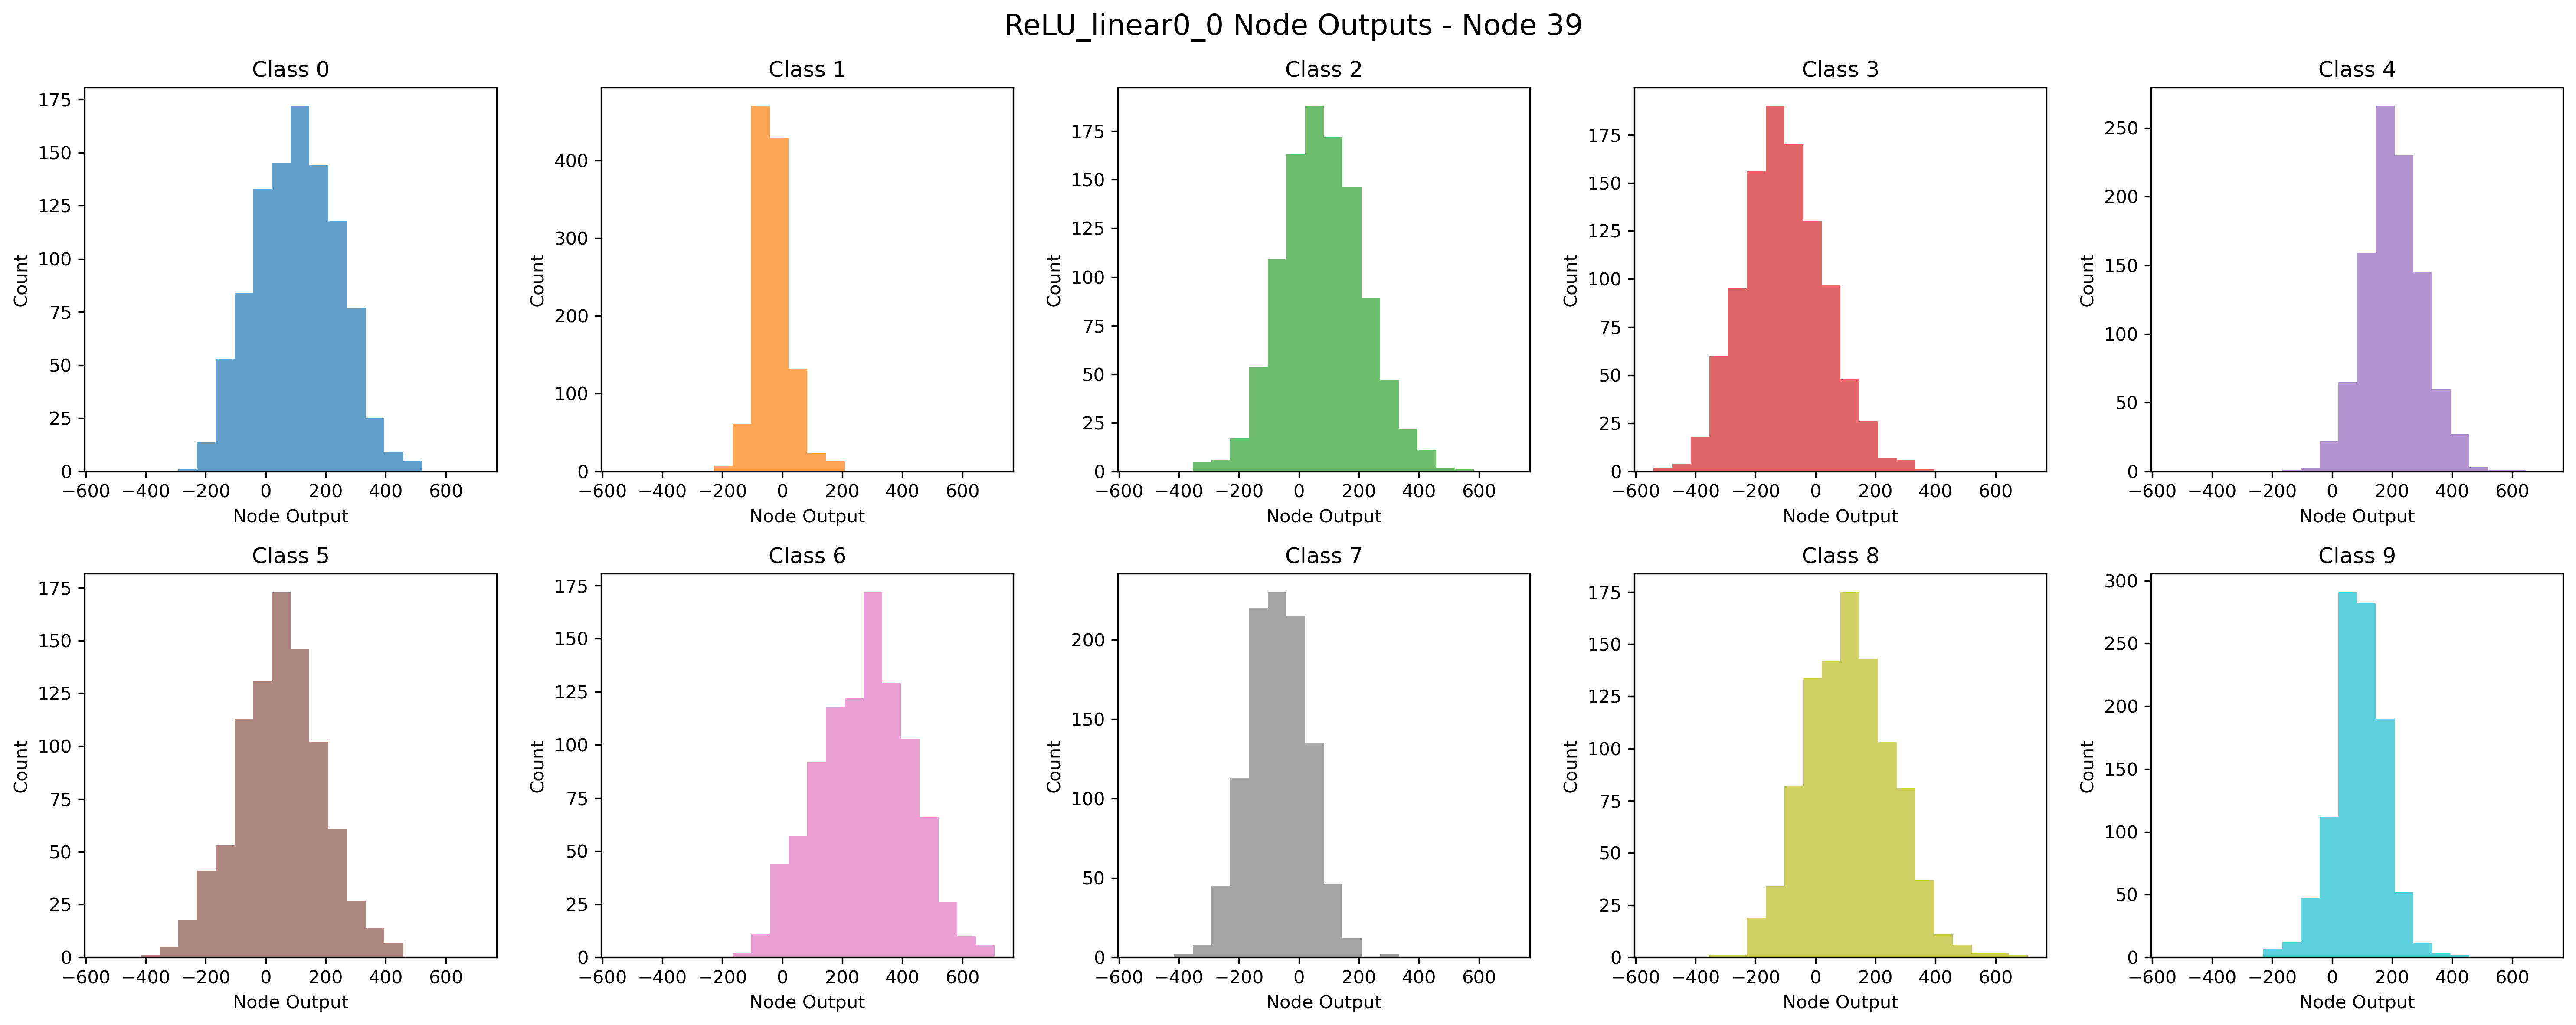
\includegraphics[width=0.4\textwidth]{images/distance_distribution}
    \caption{Class distributions in the latent space show overlapping clusters with varying statistical properties. Each class exhibits distinct characteristics (mean, variance, skewness), with overlap patterns varying across different linear projections - typical behavior for non-linearly separable data.}
    \label{fig:distance_distribution}
\end{figure}
The first linear layer's outputs form a 128-dimensional latent space, where the second layer defines a hyperplane $y=Wx+b$ ($b=0$). While traditional analysis views hyperplanes as boundaries that separate clusters, our distance-based interpretation focuses on how hyperplanes intersect clusters to define prototypes. The hyperplane is uniquely defined by 128 points: 127 points on the decision boundary (representing learned prototypes within clusters), the origin (due to $b=0$), and one point outside the latent space. These intersections with clusters determine the hyperplane's orientation and thus how the network measures distances to prototypes for classification.In this latent space, we define two important points for each class $c$: an optimal center $z_c$ that minimizes intra-class distances while maximizing inter-class distances, and its counterpart $z_{\neg c}$ that does the opposite. These points, constructed from the first layer's node outputs, represent ideal prototypes within their respective clusters.
When learning a distance representation, the second linear layer's hyperplane attempts to intersect points approximating $z_c$ on its decision boundary. This alignment ensures the target class has minimal activations by positioning the boundary near its ideal center, effectively identifying classes based on their proximity to these centers.
When learning an intensity representation, the second linear layer's hyperplane attempts to intersect points approximating $z_{\neg c}$ on its decision boundary. This alignment ensures the target class has maximal activations by positioning the boundary near the centers of non-target classes, effectively separating classes based on their distance from these "anti-centers."
\subsection{Analysis of ReLU-based Architectures}

\texttt{ReLU2} failed catastrophically ($47.20\% \pm 12.00\%$) due to widespread node death in its output layer: $33.00\%$ of nodes were permanently inactive and $53.50\%$ activated for less than 5\% of inputs. This failure stems from attempting to learn a disjunctive distance representation while constrained by intensity-based learning. Since non-target classes comprise 90\% of the data for any classification decision, the network drives most pre-activations negative to minimize non-target activations.

The dead node collapse emerges from a compounding effect: when classes overlap in the latent space, minimizing activations for non-target classes ($\neg c$) inevitably affects the target class ($c$) as well. Since each class comprises only 10\% of the data, the optimization overwhelmingly prioritizes minimizing non-target activations (90\% of cases) over preserving activations for the target class (10\% of cases). As a result, pre-activations for both target and non-target classes are driven negative, which the second ReLU then zeros out, leading to widespread dead nodes.

In contrast, \texttt{ReLU2-Neg} achieves near-baseline performance ($94.93\% \pm 0.15\%$) by building a conjunctive distance representation. It positions hyperplanes so that class $c$ points have negative pre-activations (centered around $z_c$), which ReLU converts to zero. Crucially, this also applies to all classes with even smaller pre-activations (i.e., those positioned to the left of $z_c$ in the projected space, as shown in Figure~\ref{fig:distance_distribution}). Since ReLU zeros out everything below the target class, the network must rely on the decorrelation of these classes across different hyperplane projections to prevent them from overlapping with the target class. The diverse projections in the latent space ensure this decorrelation, allowing the target class to maintain minimal activation while maximizing $\neg c$.

\subsection{Analysis of Abs-based Architectures}

Unlike ReLU, Abs networks cannot produce dead nodes. Instead of zeroing out negative values, Abs folds them to the positive side, ensuring all nodes remain active. Under our distance metric theory—where zero activation signifies maximum feature membership—this architectural difference leads to distinct feature representations. 

In ReLU networks, maximum feature membership extends to all input regions producing negative pre-activations, creating broader feature sets. In contrast, Abs networks achieve maximum membership only at exact decision boundary points, resulting in more focused feature sets. Since the minimum activation can correspond to either $z_c$ or $z_{\neg c}$, Abs networks provide a more direct encoding of distances to learned prototypes or anti-prototypes.

While \texttt{Abs2} performed well ($95.35\% \pm 0.17\%$), its distance-learning counterpart, \texttt{Abs2-Neg}, suffered a notable accuracy drop ($90.08\% \pm 2.56\%$) with significantly higher variance. What explains this unexpected performance gap?

We theorize that \texttt{Abs2-Neg} underperforms due to the clustered nature of MNIST, where each digit class occupies a distinct region of the input space. An output hyperplane in \texttt{Abs2-Neg} must pass through an optimal prototype point $z_c$ for the target class, along with 127 additional linearly independent points. Since there is only one ideal $z_c$ that best represents the target class, the remaining points must be suboptimal. These non-optimal points lie closer to non-target and result in misclassifications. \texttt{Abs2-Neg} is constrained to a single, rigid prototype representation, making it vulnerable to class overlap and limiting its ability to generalize.

In contrast, \texttt{Abs2} constructs its hyperplane by selecting $z_{\neg c}$, the centers of non-target classes, for each latent dimension. Since each dimension can be aligned with any of the nine non-target classes, \texttt{Abs2} has a vast combinatorial space of possible hyperplane configurations ($9^{128}$ choices). This flexibility allows it to compensate for suboptimal points in some dimensions by making better choices in others. As a result, \texttt{Abs2} can achieve robust class separation, explaining its higher accuracy and lower variance compared to \texttt{Abs2-Neg}.

\subsection{Validation Through Additional Experiments}

Our theory about the \texttt{Abs2-Neg} performance drop suggests that a layer designed to explicitly represent the distance to a single optimal point might correct the performance difference. To address the limitations of \texttt{Abs2-Neg}, where the need for multiple non-optimal intersection points hampered performance, we propose a layer called OffsetL2 that computes the weighted L2 distance from a single learned reference point $\mu$:

\[
y_i = || \alpha_i \odot (x - \mu_i) ||_2
\]

OffsetL2 directly implements our geometric intuition by explicitly learning a single optimal reference point, $\mu_i$, for each class, corresponding to the hypothesized ideal prototype $z_c$. The learnable weight vector $\alpha_i$ modulates the importance of each dimension in the distance calculation, providing greater flexibility. This approach contrasts with \texttt{Abs2-Neg}, which implicitly discovers prototypes through hyperplane positioning.

When combined with LogSoftmax, OffsetL2 shows interesting connections to established architectures:

\begin{table}[H]
    \centering
    \footnotesize
    \begin{tabular}{lc}
        \toprule
        \textbf{Method} & \textbf{Equation} \\
        \midrule
        OffsetL2 + LogSoftmax & $ y_i = \exp(-||\alpha_i \odot (x - \mu_i) ||_2) $ \\  
        Traditional RBF & $ y_i = \exp(-0.5 (\text{precision}_i (x - \mu_i)^2)) $ \\  
        Mahalanobis + LogSoftmax & $ y_i = \exp(-||\text{precision}_i v_i (x - \mu_i)||_2) $ \\  
        \bottomrule
    \end{tabular}
    \caption{Comparison of OffsetL2 with related distance-based methods.}
    \label{tab:comparison_offsetl2}
\end{table}

When preceded by a linear layer, OffsetL2 becomes functionally equivalent to the PCA-based Mahalanobis distance, where the linear layer learns principal components ($V$) and OffsetL2 learns the scaling ($\Lambda^{-1/2}$) and mean ($\mu$). This strong connection between OffsetL2, RBF networks, and Mahalanobis distance further reinforces its theoretical grounding.

To evaluate OffsetL2, we introduced four new models: \texttt{ReLU-L2}, \texttt{ReLU-L2-Neg}, \texttt{Abs-L2}, and \texttt{Abs-L2-Neg}. Training was extended to 50,000 epochs after observing that models had not fully converged at 5,000 epochs.


\begin{table}[H]
    \centering
    \footnotesize
    \begin{tabular}{lcc}
    \toprule
    \textbf{Model} & \textbf{Accuracy (\%)} & \textbf{Std Dev (\%)} \\
    \midrule
    % Baseline Models
    ReLU\_Bias & 96.62 & 0.17 \\
    ReLU2\_Bias & 56.31 & 19.31 \\
    ReLU2\_Neg & 96.46 & 0.17 \\
    Abs\_Bias & 95.87 & 0.22 \\
    Abs2\_Bias & 95.95 & 0.17 \\
    Abs2\_Neg\_Bias & 92.25 & 2.07 \\
    \midrule
    % OffsetL2 Models
    ReLU-L2 & 97.33 & 0.13 \\
    ReLU-L2-Neg & 97.36 & 0.14 \\
    Abs-L2 & 97.61 & 0.07 \\
    Abs-L2-Neg & 97.56 & 0.09 \\
    \bottomrule
    \end{tabular}
    \caption{Performance metrics across all models with extended training (50,000 epochs), averaged over 20 runs.}
    \label{tab:extended_training}
\end{table}

The results demonstrate several key findings:

1. The performance gap between normal and negated variants disappeared, supporting our theory about explicit prototype learning.
2. \texttt{ReLU-L2} avoided the catastrophic failure of \texttt{ReLU2\_Bias}.
3. OffsetL2 architectures significantly outperformed baselines, with \texttt{Abs-L2} models achieving $\sim 97.6\%$ accuracy.
4. All OffsetL2 models exhibited remarkably low variance ($\leq 0.14\%$).

These findings validate our theoretical framework: by explicitly modeling geometric constraints through direct distance calculations, OffsetL2 not only improves accuracy but also stabilizes training. The convergence in performance between normal and negated variants provides strong empirical validation of our core hypothesis—explicitly modeling distances to learned prototypes leads to more robust and accurate learning.

Our results, combined with geometric analysis, suggest a fundamental shift in how neural network representations should be conceptualized. Moving beyond the traditional intensity-based paradigm, these findings highlight the power of statistical distance metrics and geometric constraints, paving the way for new architectural advances in deep learning.
